\chapter{Implementation}
\label{chap:Chapter 4 title}


\section*{Introduction}
Following the methodological framework detailed in the preceding chapter, this chapter delves into the practical implementation of the Federated Learning system for Water Quality Monitoring. It provides a comprehensive account of the software components developed, the system integration strategies employed, and the specific technical choices made to bring the conceptual design to life.

The chapter begins by describing the simulation of real-time data collection, a crucial step for testing and validation in the absence of a fully deployed physical sensor network. It then elaborates on the intricacies of the data preprocessing pipeline executed on the edge devices, covering anomaly detection techniques, data cleaning, imputation models, and the notification system designed to report operational metrics.

Subsequently, the implementation of the core Federated Learning workflow is detailed, including client participation and server-side aggregation. A significant portion is dedicated to feature engineering for enhanced water quality prediction and the integration of these features into Recurrent Neural Network (RNN) models. Security, a paramount concern, is addressed through the implementation of mutual TLS (mTLS) and TLS for secure communication between system components. Finally, the chapter outlines the development of the backend infrastructure and the user-facing web interfaces both for client users and system administrators highlighting the technologies used and the functionalities provided.

\pagebreak



\section{Software Components and System Integration}

\subsection{Data Injection and Simulation}
To simulate real-time data collection from water quality monitoring robots, we relied on historical datasets containing time-series measurements of various parameters such as temperature, pH level, dissolved oxygen, turbidity, and conductivity. These datasets acted as stand-ins for actual sensor streams, allowing us to create a controlled and repeatable environment to test the local preprocessing and federated learning workflows deployed on each Raspberry Pi.

The simulation process was implemented via custom Python scripts that sequentially read data samples from CSV files and injected them into local SQLite databases hosted on each Raspberry Pi. The design aimed to mimic the behavior of real sensors pushing data in a streaming fashion, with control over the injection rate to simulate different sampling frequencies.

Each Raspberry Pi runs the injection script independently, creating a decentralized simulation environment. The data is written into a local SQLite table structured to reflect the schema expected by the preprocessing pipeline, including timestamps and all relevant water quality indicators. This modularity allowed us to test anomaly detection, cleaning, and training pipelines as if the data were being generated live.

\textbf{Pseudocode of the Simulation Process:}

\begin{algorithm}[H]
    \caption{Simulated Sensor Data Injection}
    \label{alg:sensor_injection}
    \SetAlgoLined
    \KwIn{
        Historical dataset $D$ (CSV), \\ \vspace{0.1cm}
        SQLite connection $db$, \\ \vspace{0.1cm}
        Injection interval $\Delta t$\vspace{0.1cm}
    }
    \KwOut{
        Time-series sensor data written into local SQLite database
    }
    
    \Begin{
        Initialize table schema in $db$\; \vspace{0.1cm}
        $rows \leftarrow$ read rows from $D$\; \vspace{0.1cm}
        
        \ForEach{$row \in rows$}{
            $timestamp, temperature, pH, oxygen, turbidity, conductivity \leftarrow row$\; \vspace{0.1cm}
            Insert $row$ into SQLite table\; \vspace{0.1cm}
            Sleep for $\Delta t$ seconds to simulate real-time input\; \vspace{0.1cm}
        }
    }
\end{algorithm}





\subsection{Preprocessing}
\subsubsection{Anomaly Detection}
This module aims to detect anomalous sensor readings in water quality data using three distinct methods, selected based on configuration parameters. The goal is to flag outlier values that may indicate faulty sensors, environmental issues, or data corruption.

The process begins with parsing and formatting the time field, ensuring temporal consistency. The algorithm then identifies the most frequently occurring date in the dataset, referred to as the batch\_day, which is used later for reporting and notification purposes.

Depending on the specified detection method (rule\_based, IQR, or decision\_tree), the algorithm applies one of the following techniques:

\textbf{Rule-based detection }involves checking whether each reading of pH, conductivity, temperature, or dissolved\_oxygen falls within predefined minimum and maximum acceptable.
\newline
\textbf{Interquartile Range (IQR)} method calculates the first (Q1) and third (Q3) quartiles for each numeric column. It then determines the IQR (Q3 - Q1) and flags values that fall outside the range [Q1 - 1.5×IQR, Q3 + 1.5×IQR], which are considered statistical outliers.

\textbf{Decision Tree method} trains a model for each target variable using the remaining variables as predictors. Any significant deviation between the actual and predicted values indicates a potential anomaly, which is flagged accordingly.

At the end of the process, the algorithm returns an updated DataFrame with boolean flags and a summary dictionary containing counts of anomalies per feature.

\begin{algorithm}[H]
    \caption{Anomaly Detection in Sensor Data}
    \label{alg:anomaly_detection}
    \KwIn{
        Raw sensor data DataFrame $D$ (columns: \texttt{time, pH, conductivity, temperature, dissolved\_oxygen}), \\
        Detection method $M$ (one of: \texttt{'rule\_based', 'IQR', 'decision\_tree'}), \\
        Configuration parameters $C$
    }
    \KwOut{
        DataFrame $D'$ with outlier flags (e.g., \texttt{pH\_outlier}), \\
        Summary statistics $S$ (counts per anomaly type)
    }
    
    \Begin{
        Initialize outlier columns in $D'$\;
        Convert \texttt{time} to datetime format\;
        $batch\_day \leftarrow$ Most frequent date in $D'$\;
        
        \Switch{$M$}{
            \Case{\texttt{'rule\_based'}}{
                \ForEach{column $c \in$ \texttt{[pH, conductivity, temperature, dissolved\_oxygen]}}{
                    $min, max \leftarrow C.\texttt{rule\_based\_params}[c]$\;
                    $D'[c\_outlier] \leftarrow (D'[c] < min) \lor (D'[c] > max)$\;
                }
            }
            \Case{\texttt{'IQR'}}{
                \ForEach{column $c \in$ numeric columns}{
                    $Q1, Q3 \leftarrow \text{quartiles of } D'[c]$\;
                    $IQR \leftarrow Q3 - Q1$\;
                    $D'[c\_outlier] \leftarrow (D'[c] < Q1 - 1.5IQR) \lor (D'[c] > Q3 + 1.5IQR)$\;
                }
            }
            \Case{\texttt{'decision\_tree'}}{
                \ForEach{target $t \in$ \texttt{[pH, conductivity, temperature, dissolved\_oxygen]}}{
                    Train Decision Tree on other features\;
                    $D'[t\_outlier] \leftarrow \text{predictions} \neq D'[t]$\;
                }
            }
        }
        Aggregate outlier counts into $S$\;
        \Return{$D'$, $S$}
    }
\end{algorithm}



% ==============================================
\subsubsection{Training Models}

This step focuses on building predictive models to estimate each water quality parameter namely pH, conductivity, temperature, and dissolved oxygen using the others as input features. For each target variable, the corresponding column is isolated, and the rest are used as predictors. The data is then split into training and testing sets. Depending on the configuration, a model is trained using the specified hyperparameters. Once trained, the model is evaluated using metrics like Mean Absolute Error (MAE) and the R\textsuperscript{2} score to assess its accuracy. The output includes a trained model for each target variable, along with its performance metrics.

\begin{algorithm}[H]
    \caption{Water Quality Model Training}
    
    \label{alg:model_training}
    
    \KwIn{
        Preprocessed data $D$, \\
        Model type $T$ (\texttt{KNN}, \texttt{RandomForest}, or \texttt{SVM}), \\
        Hyperparameters $H$
    }
    
    \KwOut{
        Trained models $M$ (one per target variable), \\
        Performance metrics $P$ (MAE, R2 scores)
    }
    
    \Begin{
        \ForEach{target $t \in$ \texttt{[pH, conductivity, temperature, dissolved\_oxygen]}}{
        
            $X \leftarrow D[\text{other targets}]$\;
            
            $y \leftarrow D[t]$\;
            
            Split $X,y$ into train/test sets\;
            
            $M[t] \leftarrow \text{Train } T \text{ with } H \text{ on } (X_{train}, y_{train})$\;
            
            $P[t] \leftarrow \text{Compute MAE and R2 on } (X_{test}, y_{test})$\;
        }
        \Return{$M$, $P$}
    }
\end{algorithm}



% ==============================================

\subsubsection{Imputation}
In the data preprocessing stage, sensor malfunctions were identified by treating zero values (such as a pH of 0, which is not physically plausible for water) as well as NaN entries in key water quality parameters as indicators of sensor malfunction or data corruption. These values, which had no neighboring values close to 0 to suggest a natural trend, were standardized by replacing them with NaN to ensure consistency across the dataset. A summary report was generated to quantify the number of missing or invalid entries per parameter. Subsequently, missing values were imputed using a basic statistical method, typically by substituting the mean of each respective parameter.

\begin{algorithm}[H]
    \caption{Missing Data Imputation}
    \label{alg:imputation}
    \KwIn{
        Raw data $D$ with possible missing/zero values, \\
        Imputation strategy $S$ (default: \texttt{mean})
    }
    \KwOut{
        Imputed DataFrame $D'$, \\
        Report $R$ of missing/zero counts per column
    }
    
    \Begin{
        Initialize $R$ as empty dictionary\;
        
        \ForEach{column $c \in$ \texttt{[pH, conductivity, dissolved\_oxygen]}}{
        
            $R[c] \leftarrow \left\{
                \begin{array}{ll}
                    \texttt{nan\_count}: & \text{count of } \texttt{NaN}, \\
                    \texttt{zero\_count}: & \text{count of } 0
                \end{array}
            \right\}$\;
            
            Replace $0$s with $\texttt{NaN}$ in $D'[c]$\;
            
        }
        Fit \texttt{SimpleImputer} with strategy $S$ on $D'$\;
        
        Transform $D'$ with imputed values\;
        
        \Return{$D'$, $R$}
    }
\end{algorithm}

% ==============================================
\subsubsection{Notification}
The notification mechanism is designed using a decorator-based monitoring system. This pattern allows monitoring logic to be automatically injected into any function it decorates, without altering the core logic of the function itself. When a decorated function such as anomaly detection, model training, or missing value handling is called, the system first prepares metadata including the batch date extracted from the input data. Once the function is executed, it returns both the result and relevant metadata. Based on the step type, the system constructs a payload that includes relevant information: the number of detected outliers, model performance metrics, or missing value statistics. This payload is then sent to a remote monitoring server via HTTPS, ensuring that the execution of each step is logged and observable in real time.

\begin{algorithm}[H]
\caption{Decorator-Based Monitoring System}
\label{alg:monitoring}
\SetAlgoLined
\DontPrintSemicolon

\KwIn{
    Decorated function $f$ with parameters \texttt{*args, **kwargs}\;
    Step name $step\_name$ (e.g., "Anomaly Detection")\;
    Configuration manager $config\_manager$\;
    Database manager $db\_manager$\;
}

\KwOut{
    Original function's return value $result$\;
    
    Monitoring payload $P$ sent to server\;
    
}

\Begin{
    \textsc{Pre-execution:}\;
    
    \Indp
    
    $batch\_day \leftarrow$ Extract most frequent date from input data\;
    
    Initialize empty metadata dictionary $meta \leftarrow \{\}$\;
    
    \Indm
    
    \textsc{Function Execution:}\;
    
    \Indp
    
    $result, meta \leftarrow f(\text{\texttt{*args, **kwargs}})$ \tcp*{Original function call}
    
    \Indm
    
    \textsc{Post-execution:}\;
    
    \Indp
    
    Construct payload $P \leftarrow \{\texttt{"step"}: \$step\_name\$, \texttt{"batch\_day"}: \$batch\_day\$\}$\;
    
    \uIf{$step\_name$ == "Anomaly Detection"}{
    
        $P[\texttt{"outliers"}] \leftarrow meta[\texttt{"outlier\_count"}]$\;
        
    }
    
    \uElseIf{$step\_name$ == "Model Training"}{
    
        $P[\texttt{"metrics"}] \leftarrow meta[\texttt{"model\_Training"}]$\;
        
    }
    
    \uElseIf{$step\_name$ == "Missing Values Handling"}{
    
        $P[\texttt{"missing\_values"}] \leftarrow meta[\texttt{"missing\_value"}]$\;
        
    }
    
    Send $P$ to monitoring server via HTTPS\;
    
    \Indm
    
    \Return{$result$}
    
}
\end{algorithm}

\subsubsection{Preprocessing Service Main Loop}

In parallel, a preprocessing service continuously monitors a raw data source at defined time intervals. It initializes required services such as a configuration manager, database handler, and processing pipeline. At each polling cycle, it fetches the latest data, updates configurations, and determines whether new data needs to be processed. If processing is needed, the system uses the last known clean date to filter and process fresh records. The clean data is then stored, and the system waits for the next cycle. If an error occurs, it is handled gracefully using exponential backoff strategies, allowing the service to recover while avoiding overwhelming the system. This fault-tolerant and modular design ensures up-to-date monitoring and continuous processing of data in a robust and scalable manner.
\begin{algorithm}[H]
\caption{Preprocessing Service Main Loop}
\label{alg:preprocessing}
\SetAlgoLined
\DontPrintSemicolon

\KwIn{
    Configuration URL $config\_url$\;
    
    Raw database path $raw\_db\_path$\;
    
    Clean database path $clean\_db\_path$\;
    
    Polling interval $\Delta t$\;
}

\Begin{

    Initialize services:\;
    
    \Indp
    $config\_manager \leftarrow \text{ConfigManager}(config\_url)$\;
    
    $db\_manager \leftarrow \text{DatabaseManager}(raw\_db\_path, clean\_db\_path)$\;
    
    $processor \leftarrow \text{WaterQualityPipeline}(config\_manager.\text{get\_config}())$\;
    
    \Indm
    
    $error\_count \leftarrow 0$\;
    
    $max\_errors \leftarrow 5$\;
    
    \While{True}{
        \Try{
            Update configuration from $config\_manager$\;
            
            $raw\_data \leftarrow db\_manager.\text{fetch\_data}()$\;
            
            \If{insufficient data}{
                Sleep for $\Delta t$ seconds\;
                
                \Continue\;
            }
            
            $last\_update \leftarrow \text{get\_last\_clean\_date}(db\_manager)$\;
            
            $clean\_data \leftarrow processor.\text{process\_data}(raw\_data, last\_update)$\;
            
            \If{$clean\_data$ not empty}{
                $db\_manager.\text{save\_clean\_data}(clean\_data)$\;
            }
            
            $error\_count \leftarrow 0$\;
            
            Sleep for $\Delta t$ seconds\;
        }
        
        \Catch{KeyboardInterrupt}{
            \Break\;
        }
        
        \Catch{Exception $e$}{
            Handle error with exponential backoff\;
        }
    }
}

\end{algorithm}






\subsection{Federated Learning}

The system employs a federated learning (FL) approach, detailed in Chapter [\ref{chap:Chapter 3 title} (Methodology), for privacy-preserving, distributed model training. In essence, a central server coordinates Raspberry Pi clients, which train a global WQI prediction model on their local data. Only model updates, not raw data, are exchanged and aggregated centrally to refine the model iteratively, ensuring data privacy and security.

\subsubsection{Feature Selection for Enhanced Water Quality Prediction}
Selected features capture essential water quality aspects and temporal dynamics, emphasizing core parameters and their behavior over short and medium-term observation windows.

\textbf{Core Environmental Parameters}

Four primary environmental parameters form the foundation of our analysis:

\begin{longtable}{p{3.5cm}p{10cm}}
\caption{Core Water Quality Parameters and Their Roles} \\
\toprule
\textbf{Parameter} & \textbf{Role in Water Quality Assessment} \\
\midrule
\endfirsthead

\toprule
\textbf{Parameter} & \textbf{Role in Water Quality Assessment} \\
\midrule
\endhead

\midrule
\multicolumn{2}{r}{\small\itshape Continued on next page} \\
\midrule
\endfoot

\bottomrule
\endlastfoot

\textbf{pH} &
Serves as a critical indicator of water's acidity or alkalinity, directly influencing aquatic ecosystem health and chemical processes. \\
\midrule

\textbf{Temperature} &
Acts as a fundamental driver of biochemical reaction rates and significantly impacts dissolved oxygen solubility. \\
\midrule

\textbf{Dissolved Oxygen (DO)} &
Represents the water's capacity to support aquatic life and maintain ecological balance. \\
\midrule

\textbf{Conductivity} &
Provides insights into total ion concentration, serving as an indirect indicator of pollution levels and dissolved solids. \\
\end{longtable}


\textbf{Temporal Feature Engineering}

 To account for temporal variability, time-based features were integrated into the analysis. Seasonal indicators, such as month and week of the year, were used to capture recurring patterns and contextualize fluctuations in parameter values. Rolling window statistics—specifically 7-day averages to capture short-term trends and 30-day standard deviations to reflect medium-term variability were employed to identify patterns across different time scales and detect potential instability. Additionally, percentage change metrics over 7-day and 30-day intervals were calculated to flag abrupt transitions, which may indicate pollution events, treatment effects, or natural disturbances.

\textbf{Predictive Target Integration}

Lagged Water Quality Index (WQI) features are incorporated to preserve recent historical trends, enhancing predictive power by providing context on the water quality trajectory and its connection to environmental parameters.

\begin{longtable}{|p{4cm}|p{7cm}|p{5cm}|}
\caption{Feature Categories and Their Purpose} \\
\hline
\textbf{Feature Category} & \textbf{Specific Features} & \textbf{Purpose} \\
\hline
\endfirsthead

\hline
\textbf{Feature Category} & \textbf{Specific Features} & \textbf{Purpose} \\
\hline
\endhead

\hline
\multicolumn{3}{r}{\small\itshape Continued on next page} \\
\hline
\endfoot

\hline
\endlastfoot

\textbf{Core Parameters} &
pH, temperature, dissolved\_oxygen, conductivity &
Fundamental water quality indicators \\
\hline

\textbf{Temporal Markers} &
month, week\_of\_year &
Seasonal pattern \newline identification \\
\hline

\textbf{Short-term Trends} &
pH\_7d\_avg, temperature\_7d\_avg, dissolved\_oxygen\_7d\_avg, conductivity\_7d\_avg, WQI\_7d\_avg &
Recent condition \newline assessment \\
\hline

\textbf{Medium-term Variability} &
pH\_30d\_std, temperature\_30d\_std, dissolved\_oxygen\_30d\_std, conductivity\_30d\_std &
Stability analysis \\
\hline

\textbf{Change Indicators} &
pH\_30d\_change, temperature\_30d\_change, dissolved\_oxygen\_30d\_change, conductivity\_30d\_change, WQI\_7d\_change &
Transition and anomaly detection \\
\hline
\end{longtable}

\textbf{Integration of Features in Recurrent Neural Networks}

The feature set is structured for Recurrent Neural Networks (RNNs), processing 30-day water quality sequences to capture immediate fluctuations and gradual trends. This integration allows the RNN to recognize complex temporal patterns by combining core parameters and derived temporal features. Its recurrent connections provide memory-enhanced learning by maintaining contextual awareness of historical states for anomaly detection. The model also processes data at multiple temporal granularities using raw measurements, rolling statistics.

\begin{table}[h]
\centering
\caption{RNN Integration Details}
\begin{tabular}{|p{6cm}|p{5cm}|p{5cm}|}
\hline
\textbf{RNN Integration Aspect} & \textbf{Implementation Detail} & \textbf{Benefit} \\
\hline
Sequence Length & 30 days & Captures seasonal \newline transitions and medium-\newline term patterns \\
\hline
Feature Dimensionality & 20 carefully selected \newline features & Balanced representation \newline  without redundancy \\
\hline
Temporal Connectivity & Multi-scale features from 7-day to 30-day windows & Comprehensive trend \newline analysis at various time \newline horizons \\
\hline
State Preservation & RNN hidden state \newline maintains water quality \newline context & Improved anomaly \newline detection and trend \newline forecasting \\
\hline
\end{tabular}
\end{table}

This structured integration leverages the RNN's state maintenance for improved predictive accuracy in water quality assessment.

\subsubsection{Selected Model Architecture}

The neural network predicts the Water Quality Index (WQI) from 30-timestep sequences. Each timestep has 20 features, including core sensor measurements (pH, temperature, DO, conductivity) and engineered temporal features (rolling statistics).
% \begin{figure}[H]
%     \centering
%     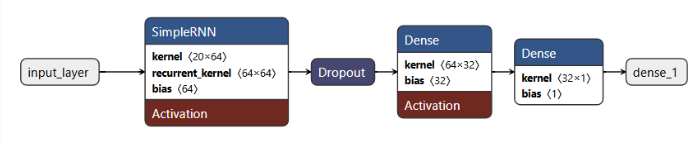
\includegraphics[width=0.75\linewidth]{Figures/RNN1.png} % Assuming this path is correct
%     \caption{Enter Caption}
%     \label{fig:enter-label-rnn1} % Made label unique
% \end{figure}

\begin{figure}[H]
    \centering
    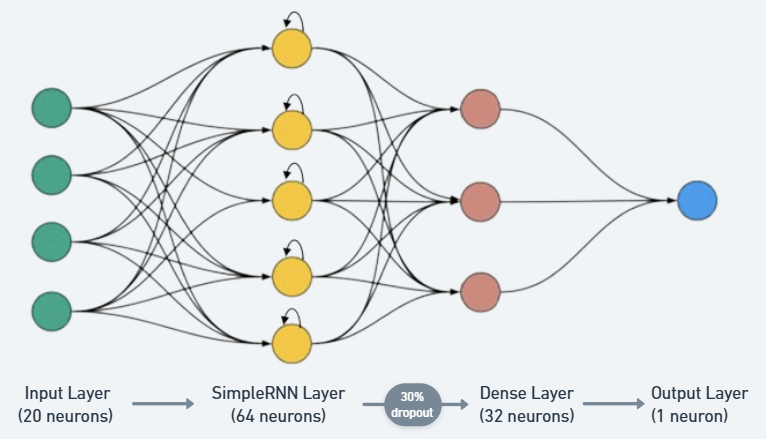
\includegraphics[width=0.75\linewidth]{Figures/RNN2.png} % Assuming this path is correct
    \caption{Enter Caption}
    \label{fig:enter-label-rnn2} % Made label unique
\end{figure}

The model's first layer is a SimpleRNN (64 neurons) that processes sequences, outputting its final hidden state as a consolidated representation. A 20\% dropout layer follows to prevent overfitting. Next, a dense layer (32 neurons, ReLU activation) refines features and reduces dimensionality. The output layer (1 neuron, linear activation) produces the continuous WQI prediction.

Data preprocessing includes robust scaling to mitigate outlier influence and ensure proportional feature contribution. Time-series sequences are generated with a 30-timestep length, enabling the model to use short-term and long-term temporal patterns. The model operates within a Flower federated learning framework for decentralized, privacy-preserving training across clients, safeguarding data and enabling collaborative learning.





\subsection{Secure Application Server Communication}

In our system, the communication between the central configuration server and the Raspberry Pi devices is secured using mutual TLS (mTLS), a protocol that ensures both the client and server authenticate each other before any data is exchanged. Unlike standard TLS, where only the client verifies the server’s identity, mTLS enforces two-way authentication, significantly strengthening security by preventing unauthorized devices from connecting to the system.

  \begin{figure}[H]
    \centering
    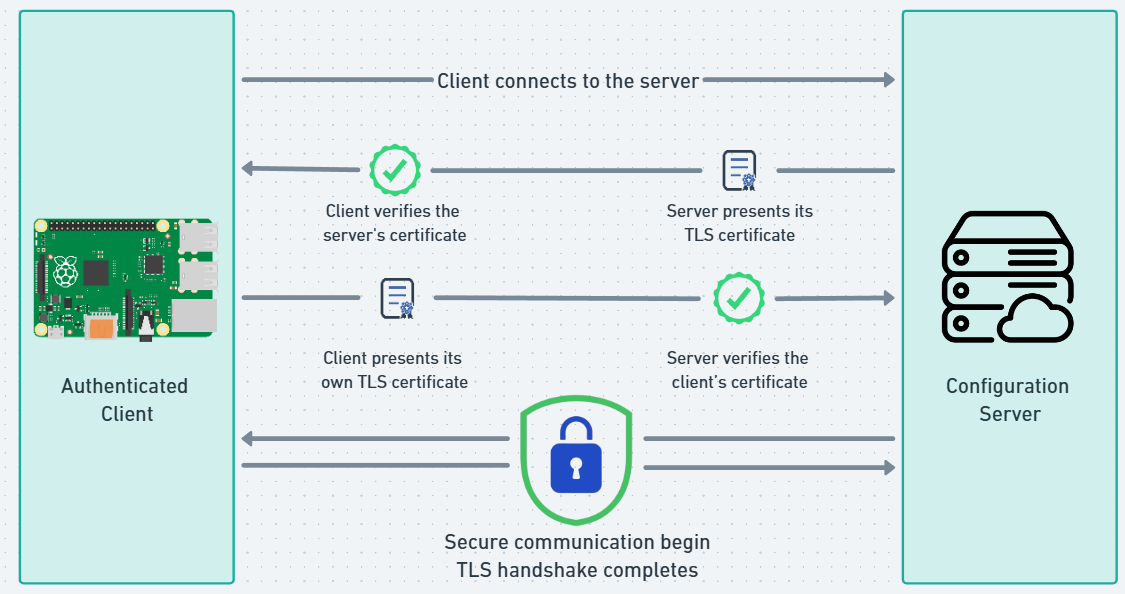
\includegraphics[width=0.75\linewidth]{Figures/mtls2.png}
    \caption{Enter Caption}
    \label{fig:enter-label}
\end{figure}

To establish this secure communication, several cryptographic files are required, including a client certificate for the Raspberry Pi, a corresponding private key, and the certificate authority (CA) certificate used to validate the trust chain. In our solution, the server is fully responsible for generating these certificates. We use a self-signed CA, maintained on the server side, to sign all client certificates.

\begin{figure}[H]
    \centering
    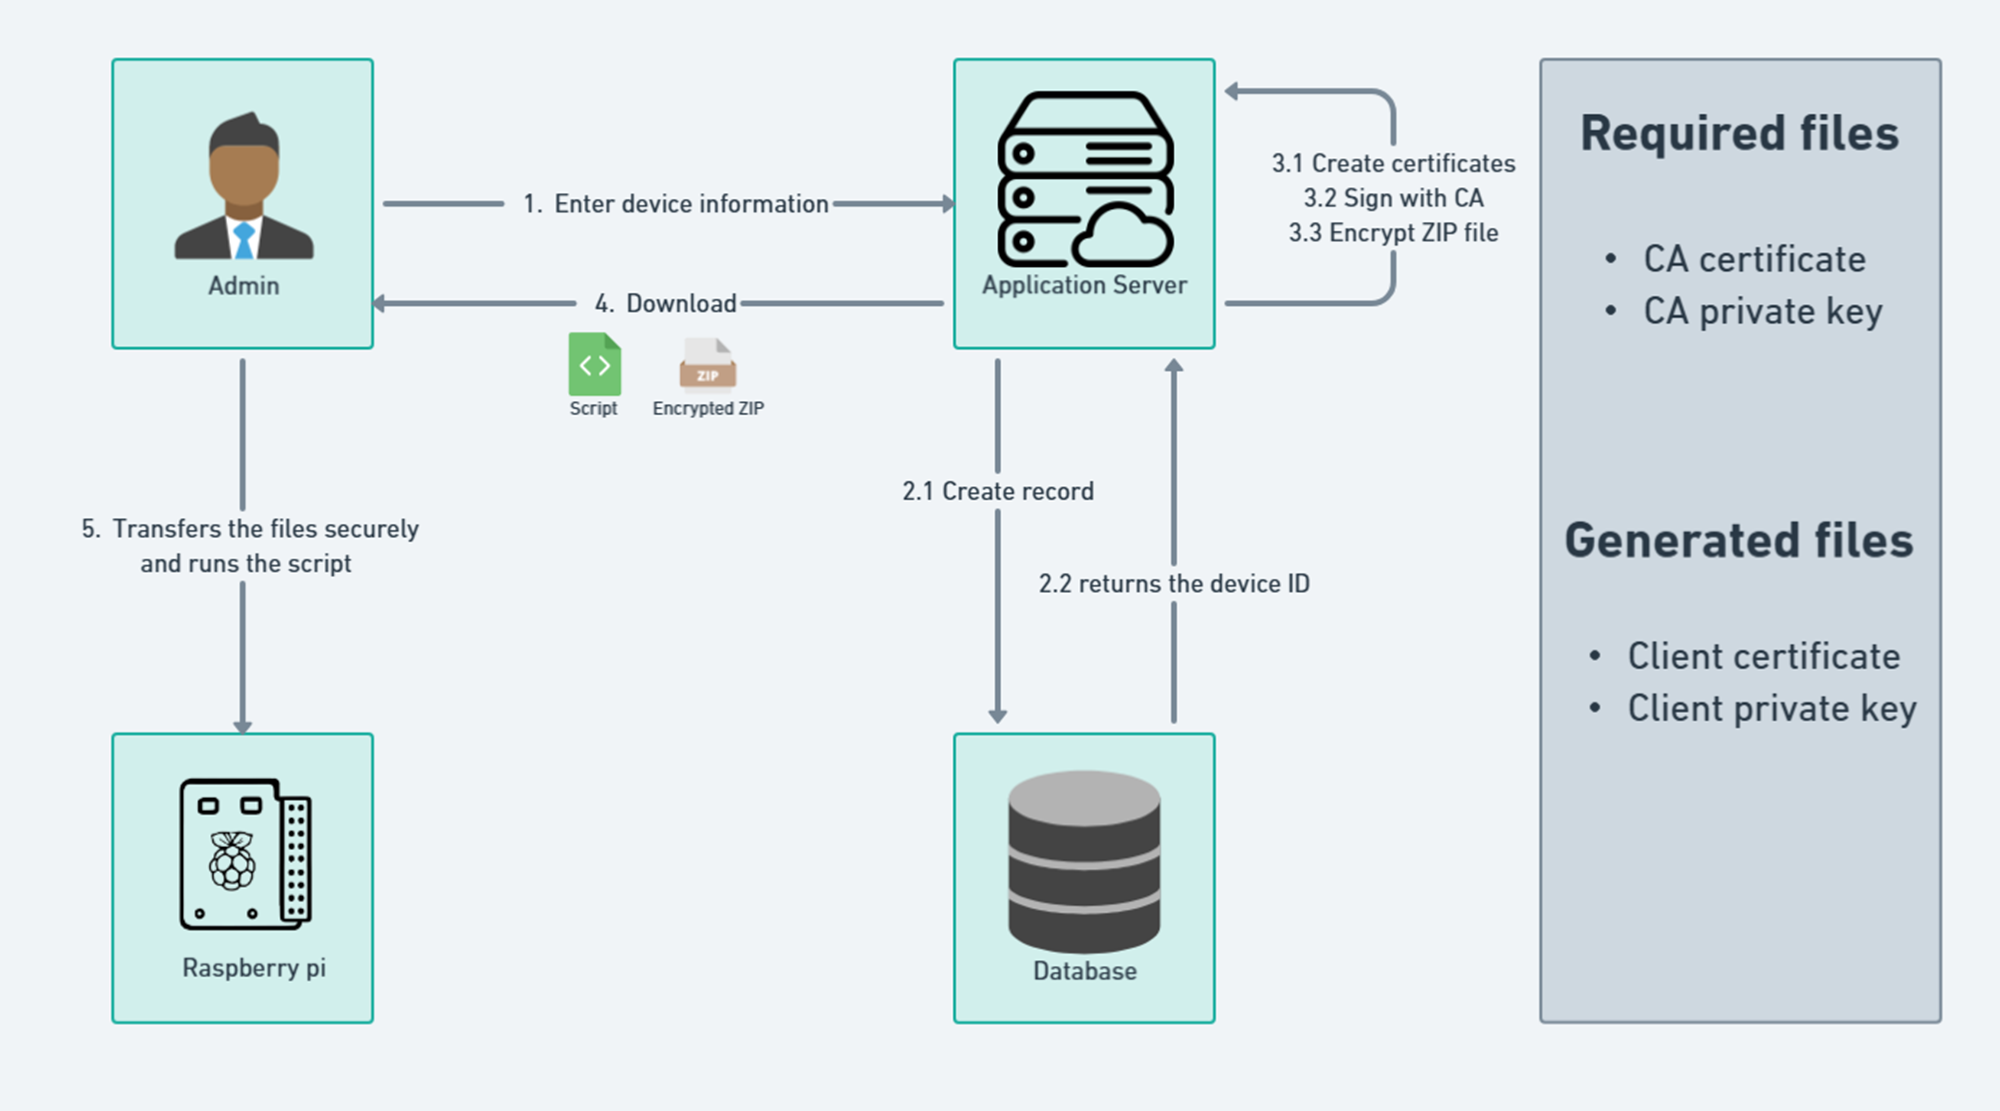
\includegraphics[width=0.75\linewidth]{Figures/security-process.png}
    \caption{Enter Caption}
    \label{fig:enter-label}
\end{figure}

The process begins when the Admin registers a new Raspberry Pi in the system. They must provide relevant information about the device, such as its region and a password. Once submitted, the server creates a new record in the database for the device. The unique ID of this record is then used as the Common Name (CN) in the certificate, ensuring each one is uniquely tied to a specific device.

The server then generates a certificate and private key for the Raspberry Pi and signs the certificate using its internal CA. These files are packaged into a password-protected ZIP archive using the password provided by the Admin. Alongside the archive, the server also generates a shell script that uses the same password and automates the installation of the certificates on the Raspberry Pi. This script simplifies the process for the Admin, allowing them to install the required certificates with minimal effort and ensuring a consistent configuration across devices.

A download link for both the ZIP archive and the installation script is provided to the Admin, who is then responsible for securely transferring them to the appropriate Raspberry Pi device. As these files contain sensitive cryptographic material, it is essential that the Admin uses secure and trusted methods to transfer them. The integrity and confidentiality of these files must be preserved during the transfer to prevent unauthorized access or compromise.



\newpage
\section{Backend and Web Interface}

\subsection{Conception}

\subsubsection{Class Diagram}
\begin{figure}[H]
    \centering
    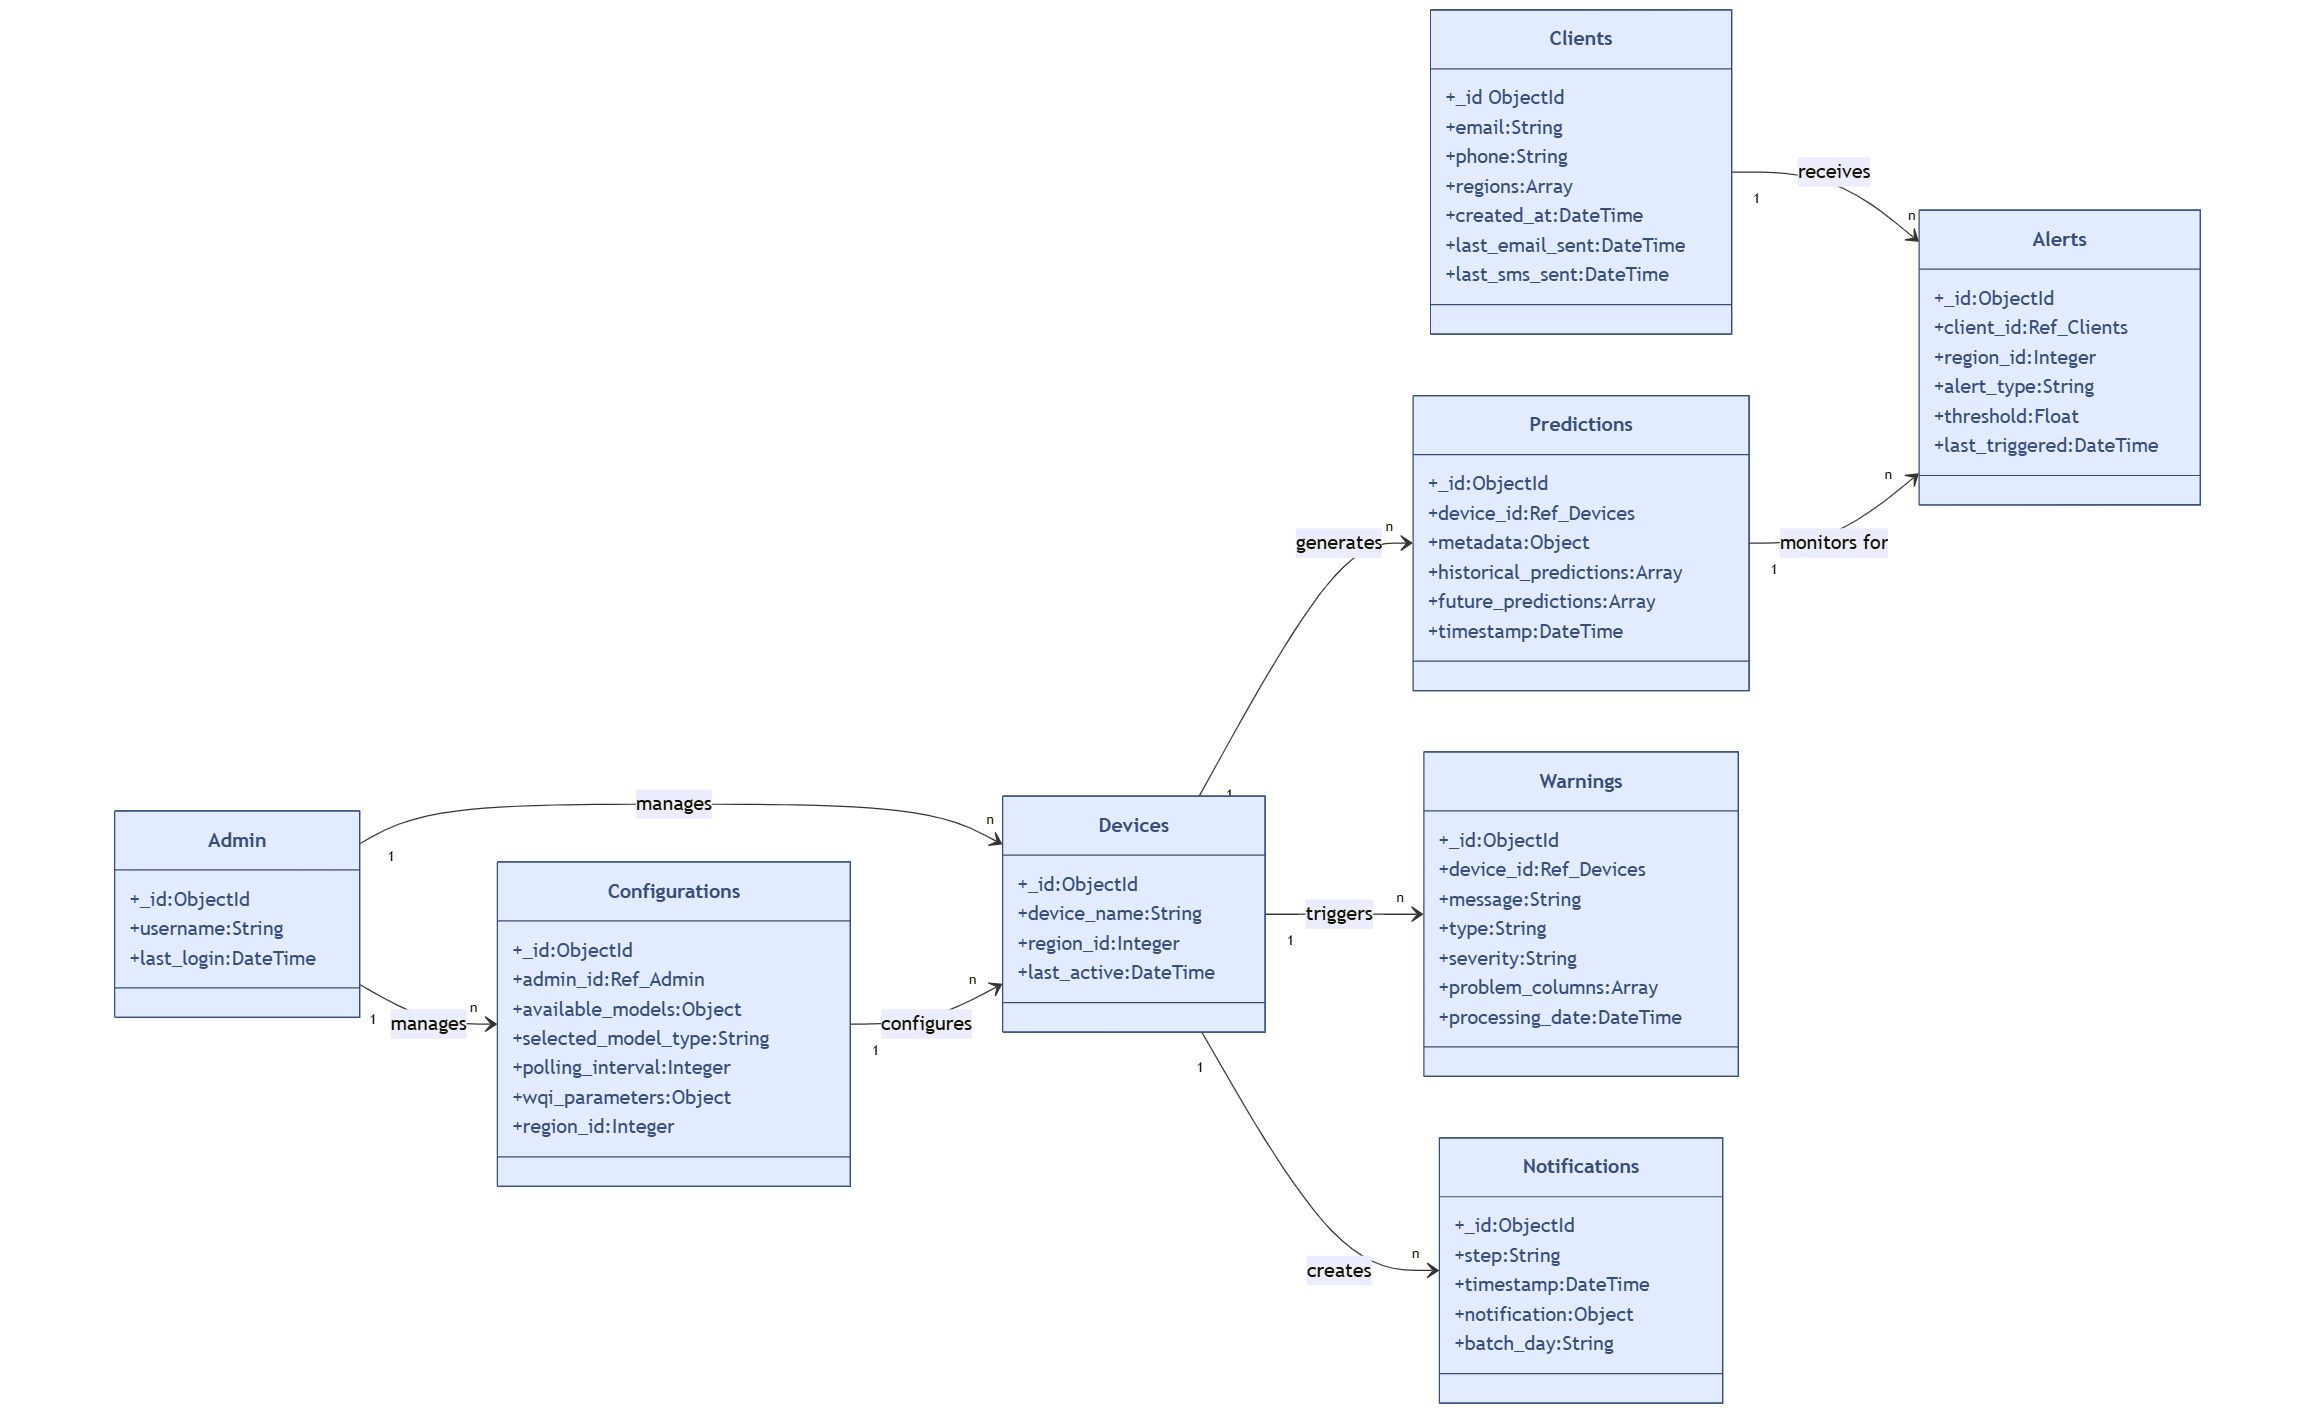
\includegraphics[width=1\linewidth]{Figures/ClasseDia.png}
    \caption{Class Diagram}
    \label{fig:enter-label}
\end{figure}
This class diagram provides an overview of the main entities involved in a monitoring and alert system, along with their relationships. The system includes key classes such as 
 \texttt{Clients}, \texttt{Devices}, \texttt{Admin}, and \texttt{Configurations}, which form the foundation of how users interact with the platform. Each class contains attributes relevant to its role for instance, the \texttt{Clients} class holds contact details and associated regions, while the \texttt{Devices} class represents the hardware responsible for collecting data. The \texttt{Admin} class is responsible for managing configurations and supervising the overall device network.

The relationships between classes illustrate the system's workflow. Devices generate \texttt{Predictions}, which may trigger \texttt{Warnings} and \texttt{Notifications} if certain thresholds are met. \texttt{Alerts} are tied to specific clients, allowing them to receive important updates when necessary. \texttt{Admins} play a central role in managing both devices and configuration settings. Additionally, predictions contribute to alert monitoring, ensuring consistent tracking and analysis of environmental or operational data.
\subsubsection{Application Architecture}
\begin{figure}[H]
    \centering
    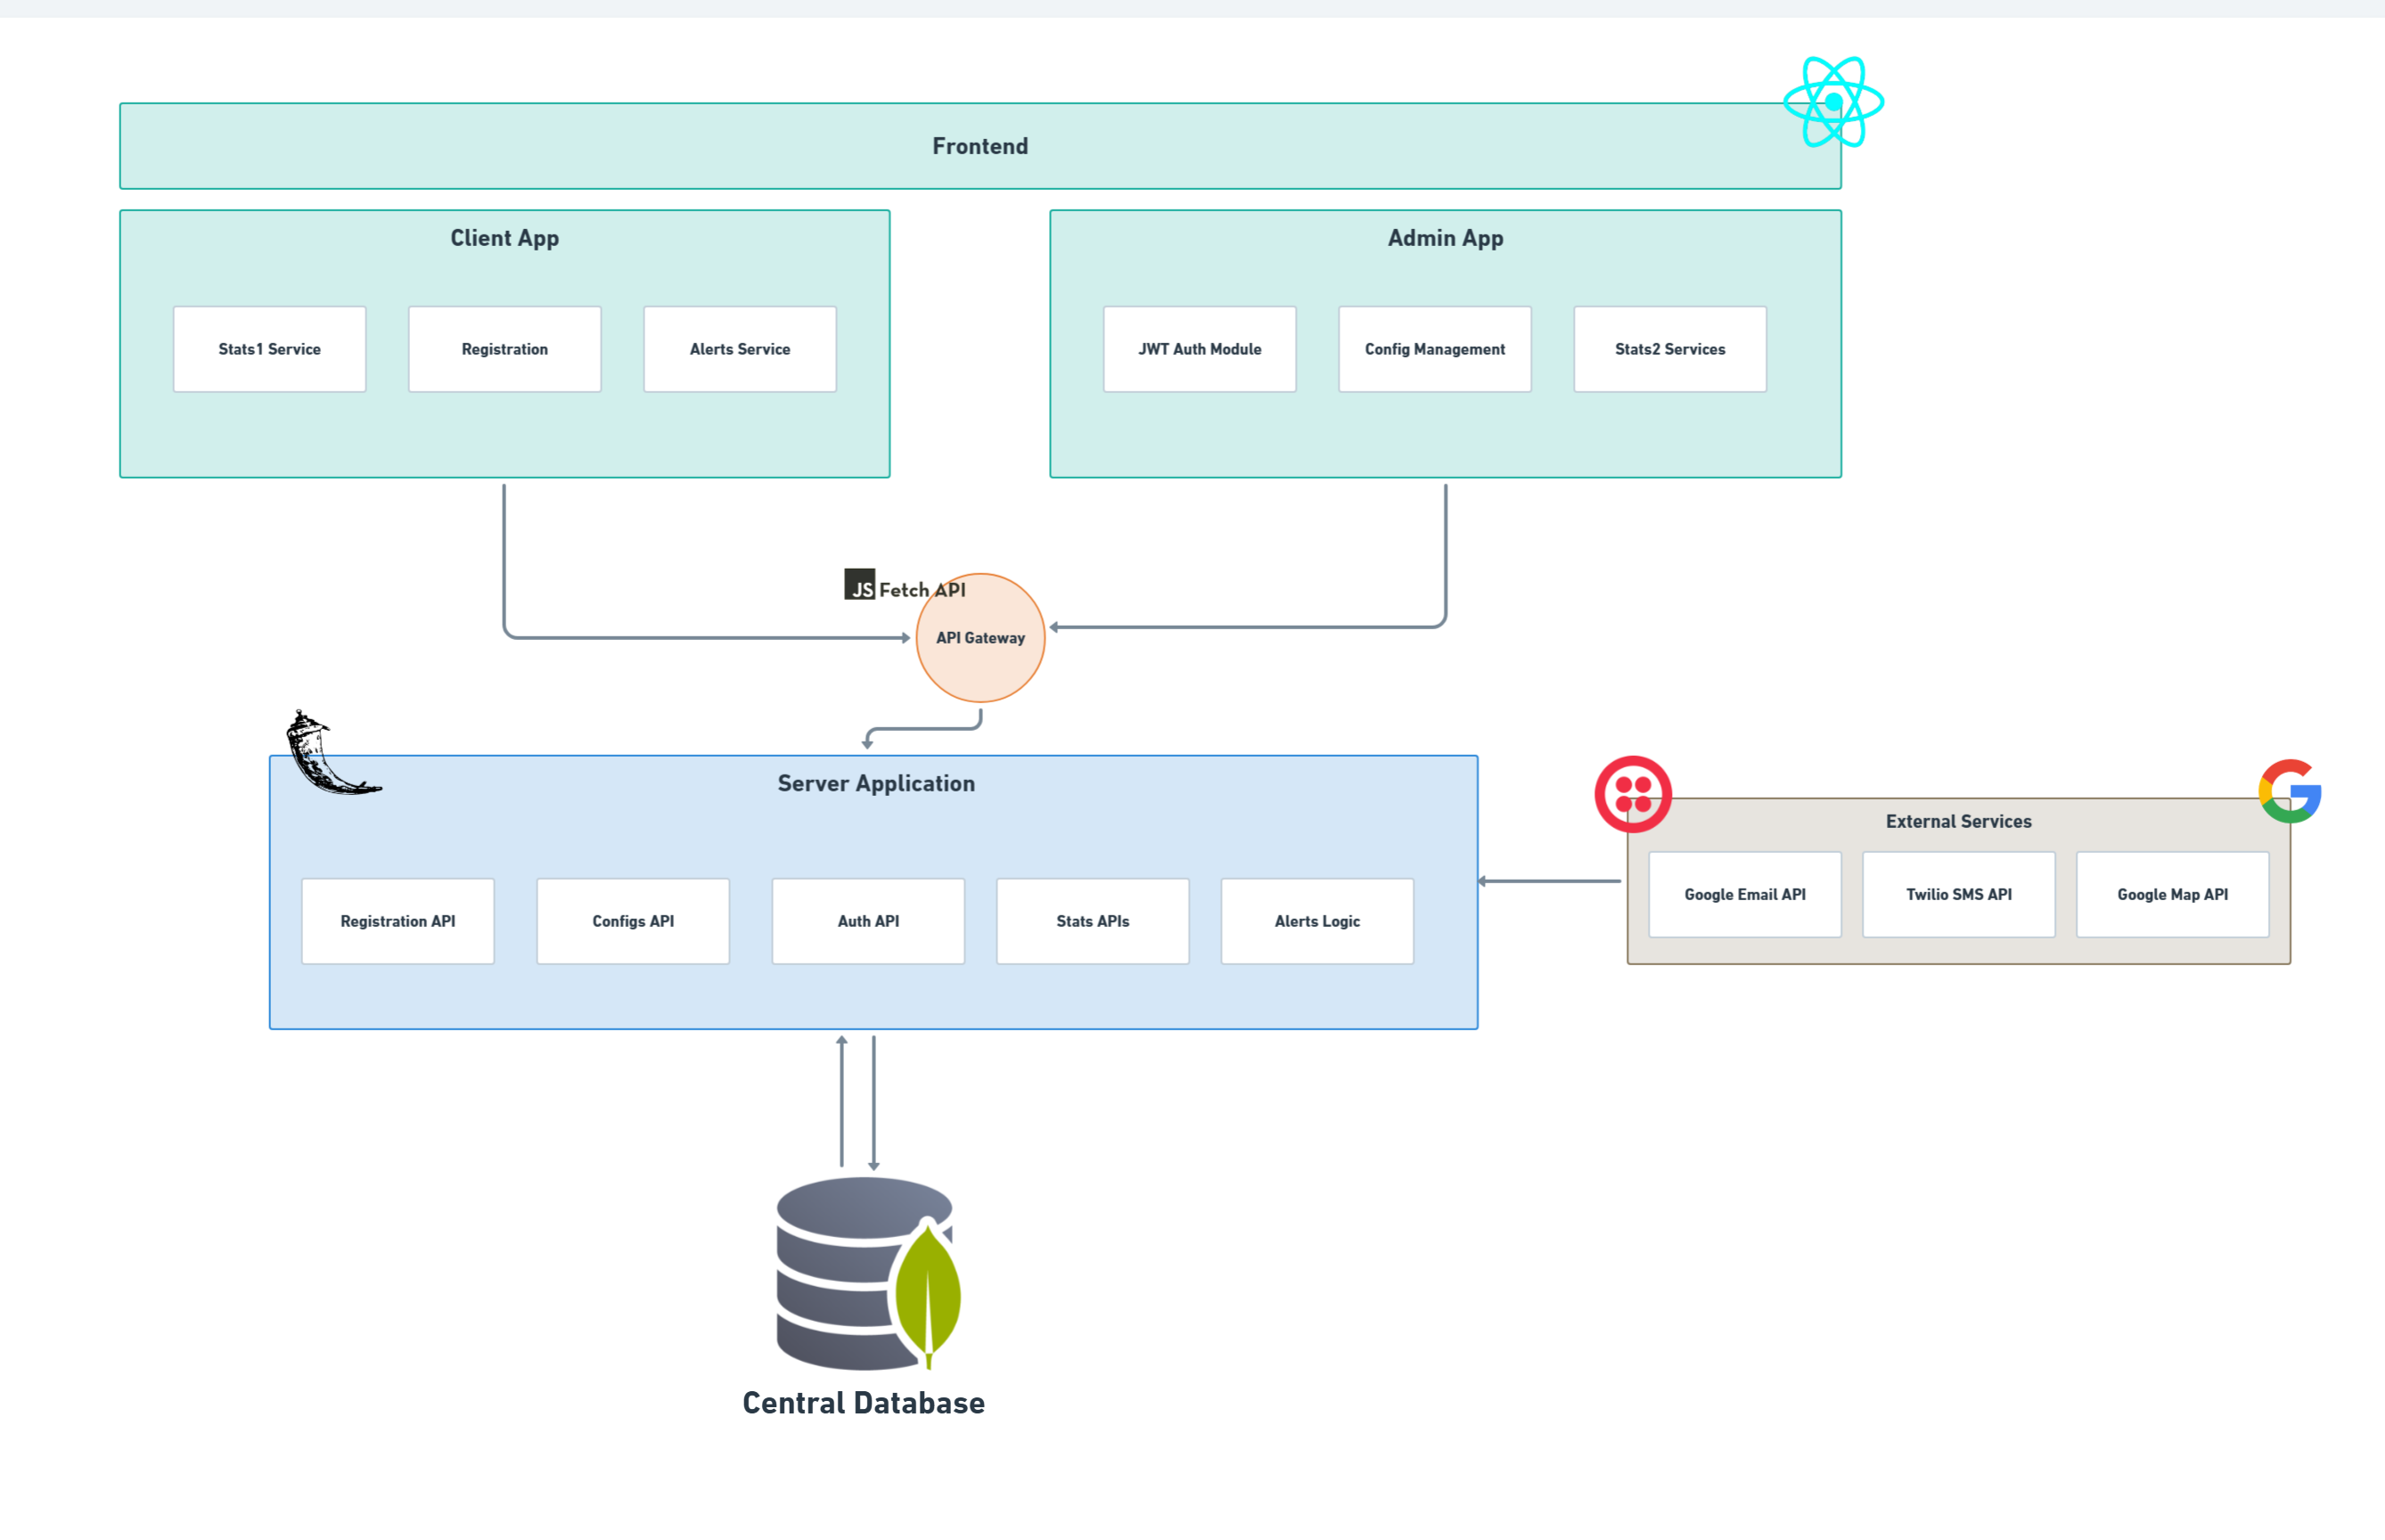
\includegraphics[width=0.75\linewidth]{Figures/ApplicatArch.png}
    \caption{Application Architecture Diagram}
    \label{fig:enter-label}
\end{figure}
The system architecture consists of two distinct React-based frontend applications: one for clients and one for administrators. The client application, built using React and JavaScript with the Fetch API for backend communication, allows users to access and monitor water quality data in major regions across Brussels. Through the \textbf{Stats1 Service}, users can view both historical and predicted Water Quality Index (WQI) values, generated using a time-series model integrated on the backend. An interactive map powered by the Google Maps API displays the current WQI levels for each location. Clients can register using their email, phone number, and select the regions they wish to track. If there is a significant drop in water quality, the system sends alerts via Twilio (for SMS) and Google Email API (for email).

The admin application, also developed with React and securely authenticated via a JWT-based module, provides a detailed operational dashboard for system managers. It interacts with a backend built using Flask, exposing multiple APIs that serve data to the frontend and communicate with Raspberry Pi devices deployed in the field. The dashboard \textbf{Stats2 Service} displays performance statistics such as the number of anomalies detected per day, total data samples, robot distribution by region, and data integrity ratios to help identify malfunctioning devices. It also presents model accuracy metrics related to federated learning (FL), and accuracy readings for pH, conductivity, and other relevant metrics. A configuration management module enables admins to remotely update detection thresholds or cleaning rules on edge devices through Flask APIs. The visualization module avoids raw sensor dumps, instead presenting actionable insights like anomaly alerts and system health indicators.




\subsection{Frontend Dashboard (React.js)}
\subsubsection{Client Application}
\begin{figure}[H]
    \centering
    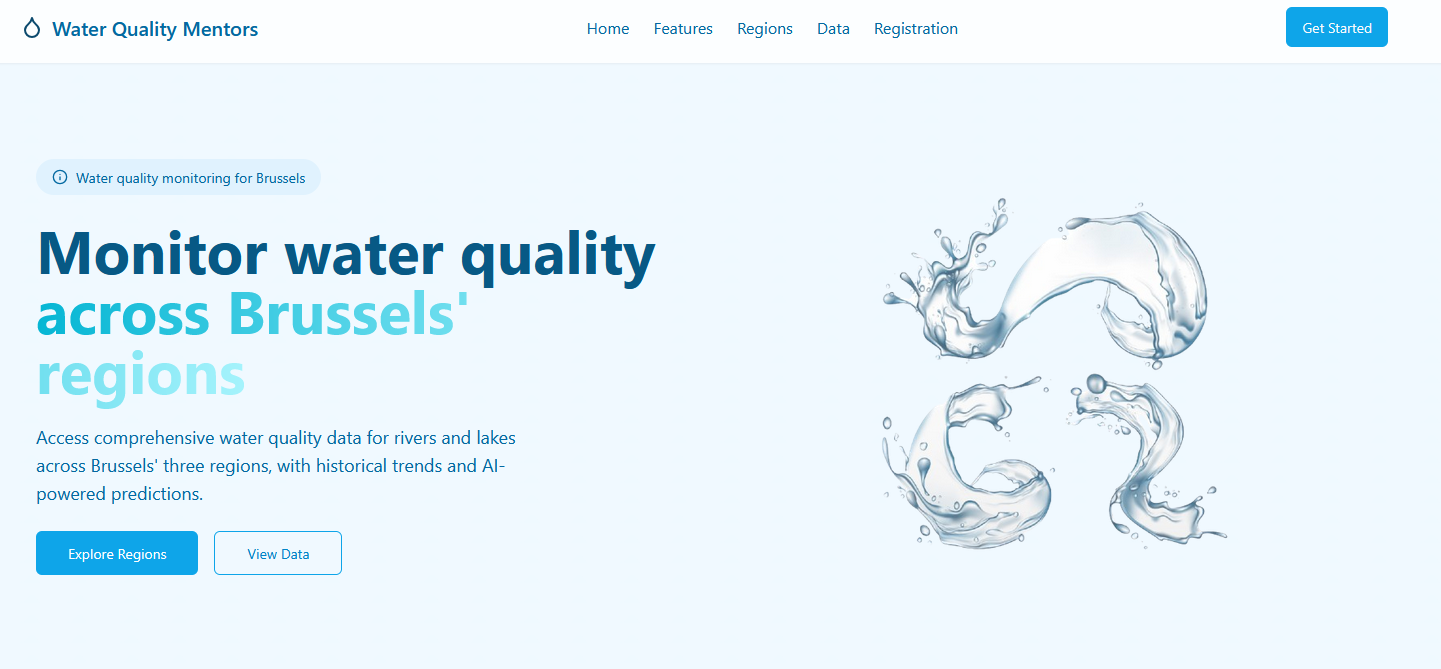
\includegraphics[width=0.75\linewidth]{Figures/clientpart1.png}
    \caption{Introduction}
    \label{fig:enter-label}
\end{figure}
This is a section of a webpage. It shows a light blue-themed header with a logo and nav links, a main title about monitoring water quality in Brussels, a short description below it, two buttons ("Explore Regions" and "View Data"), and a water splash on the left side .
\begin{figure}[H]
    \centering
    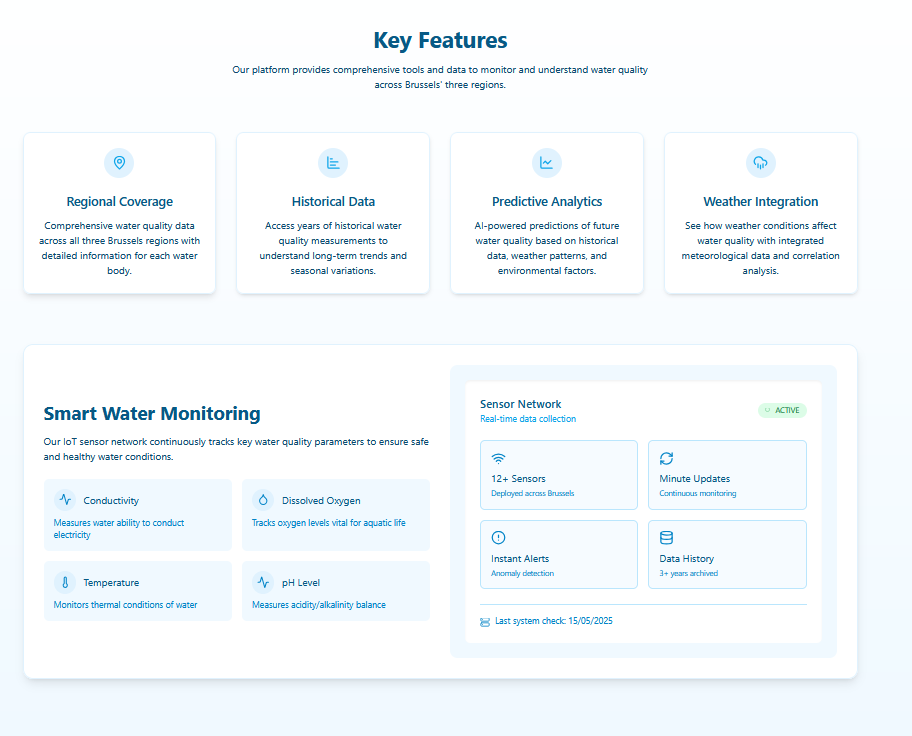
\includegraphics[width=0.75\linewidth]{Figures/clientpart2.png}
    \caption{Key Features and Info}
    \label{fig:enter-label}
\end{figure}
This is a section of a webpage titled Key Features. It presents four main features: Regional Coverage, Historical Data, Predictive Analytics, and Weather Integration each shown in separate cards with icons and short descriptions.

Below, there's a Smart Water Monitoring section describing how an IoT sensor network tracks water quality. It lists parameters like Conductivity, Temperature, Dissolved Oxygen, and pH Level. On the right, a card labeled Sensor Network shows real-time data features such as sensor count, update frequency, alerts, and data history.
\begin{figure}[H]
    \centering
    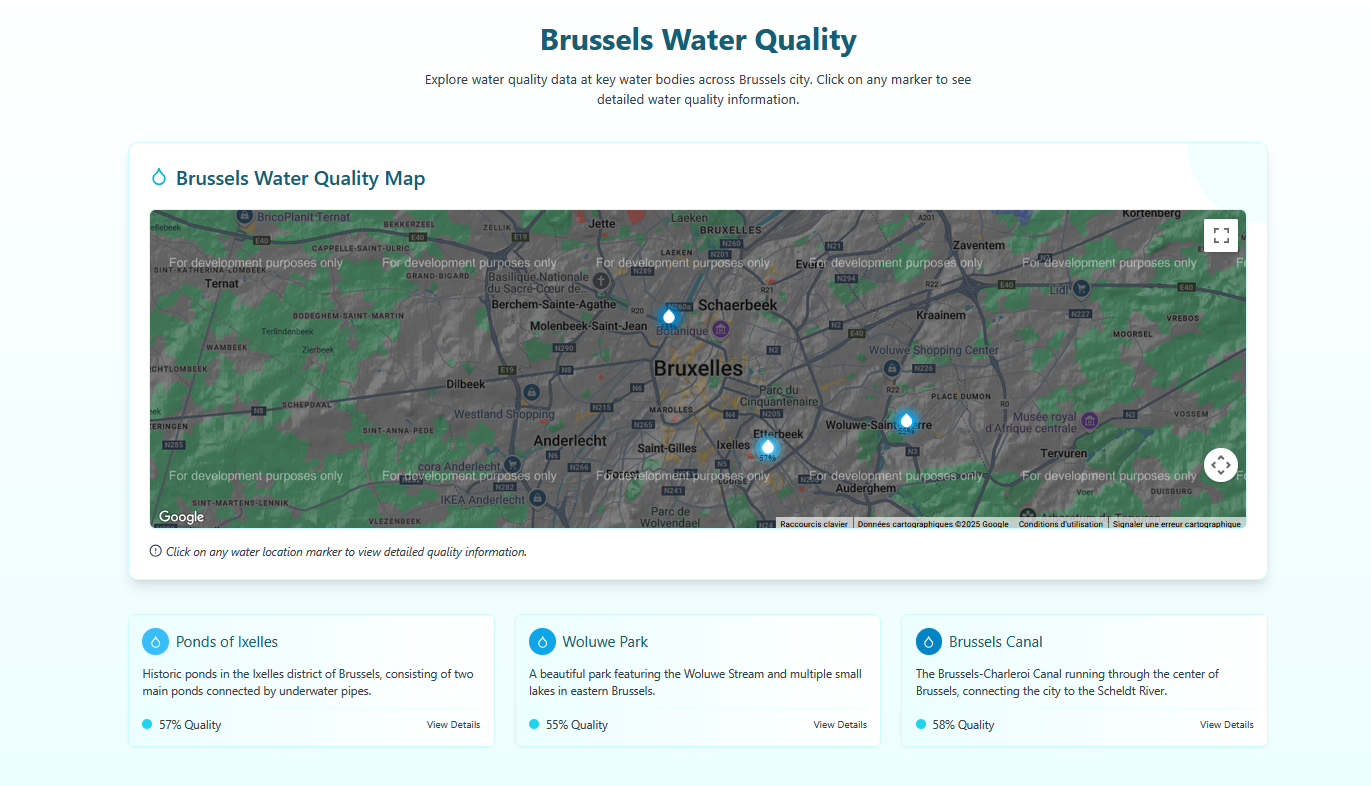
\includegraphics[width=0.75\linewidth]{Figures/clientt4.png}
    \caption{Map Feature Part 1}
    \label{fig:enter-label}
\end{figure}
The page presents an interactive map interface for Brussels water quality, using clickable pin markers and corresponding cards below the map to display information. When a user clicks on a pin or a card, a modal appears, and selecting a card also zooms the map to that specific location.
\begin{figure}[H]
    \centering
    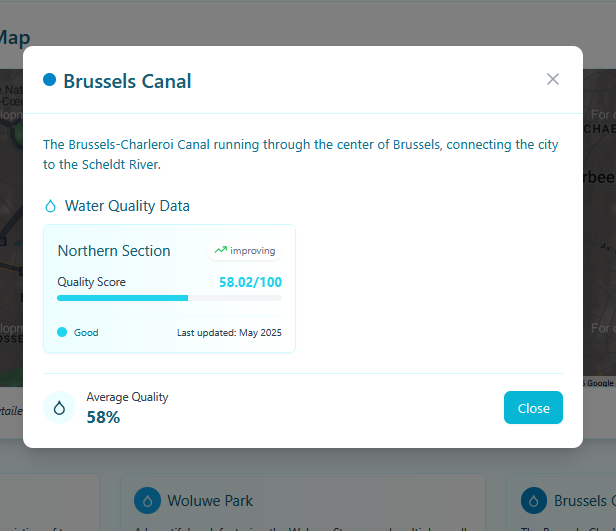
\includegraphics[width=0.75\linewidth]{Figures/clientt5.png}
    \caption{Map Feature Part 2}
    \label{fig:enter-label}
\end{figure}
When the client clicks on a specific marker on the map or selects one of the location cards, a modal is triggered. This modal presents detailed information about the selected location within one of the regions. The modal includes the Water Quality Index (WQI), the historical trend of water quality, and a brief contextual description of the location.
\begin{figure}[H]
    \centering
    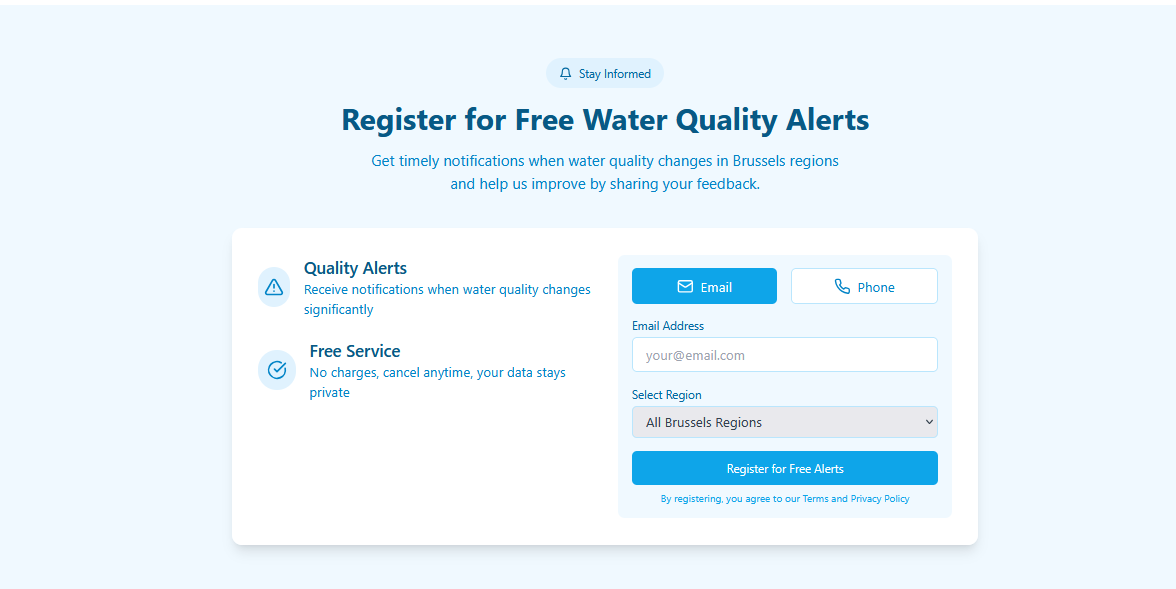
\includegraphics[width=0.75\linewidth]{Figures/clientpart8.png}
    \caption{Registration}
    \label{fig:enter-label}
\end{figure}
This registration form allows clients to subscribe to free water quality alerts via email, phone. Users can specify which Brussels regions they want to monitor. The system will then send timely notifications through Twilio for SMS and the Google Email API whenever a significant drop in water quality is detected in their selected regions, keeping them informed in real-time without constant app monitoring.
\begin{figure}[H]
    \centering
    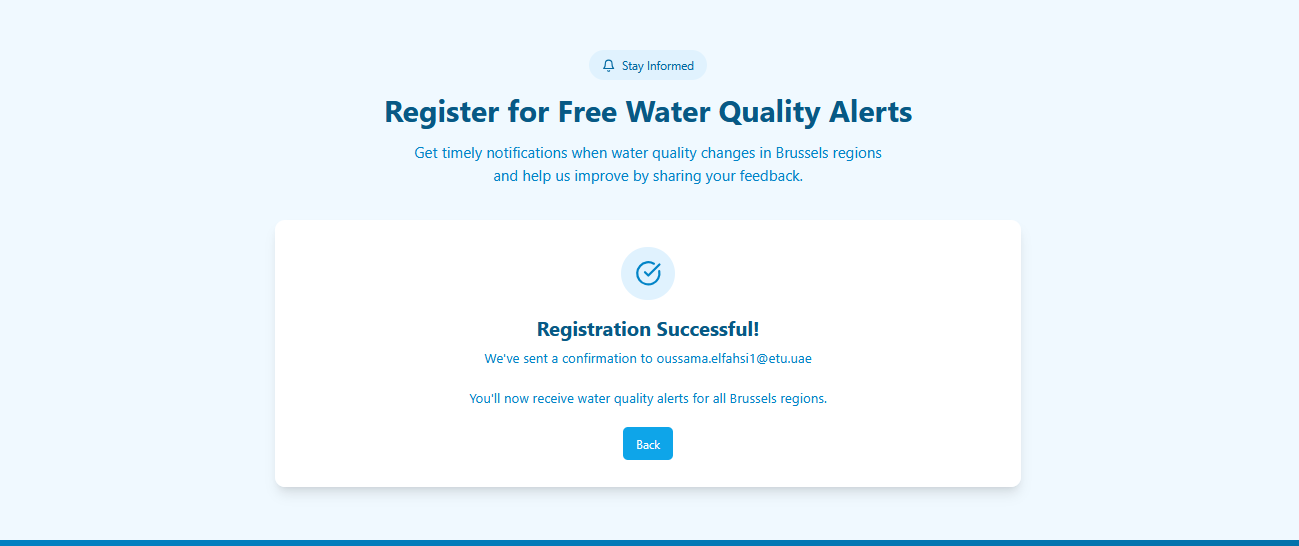
\includegraphics[width=0.75\linewidth]{Figures/Clientpartfinal.png}
    \caption{Post-Registration}
    \label{fig:enter-label}
\end{figure}
Upon successful registration, the user receives confirmation that they will now receive water quality alerts for their selected regions. A confirmation email is also sent to the provided address, ensuring the user is aware of their subscription and can expect to receive timely notifications about significant water quality changes.
\subsubsection{Admin Application}
\begin{figure}[H]
    \centering
    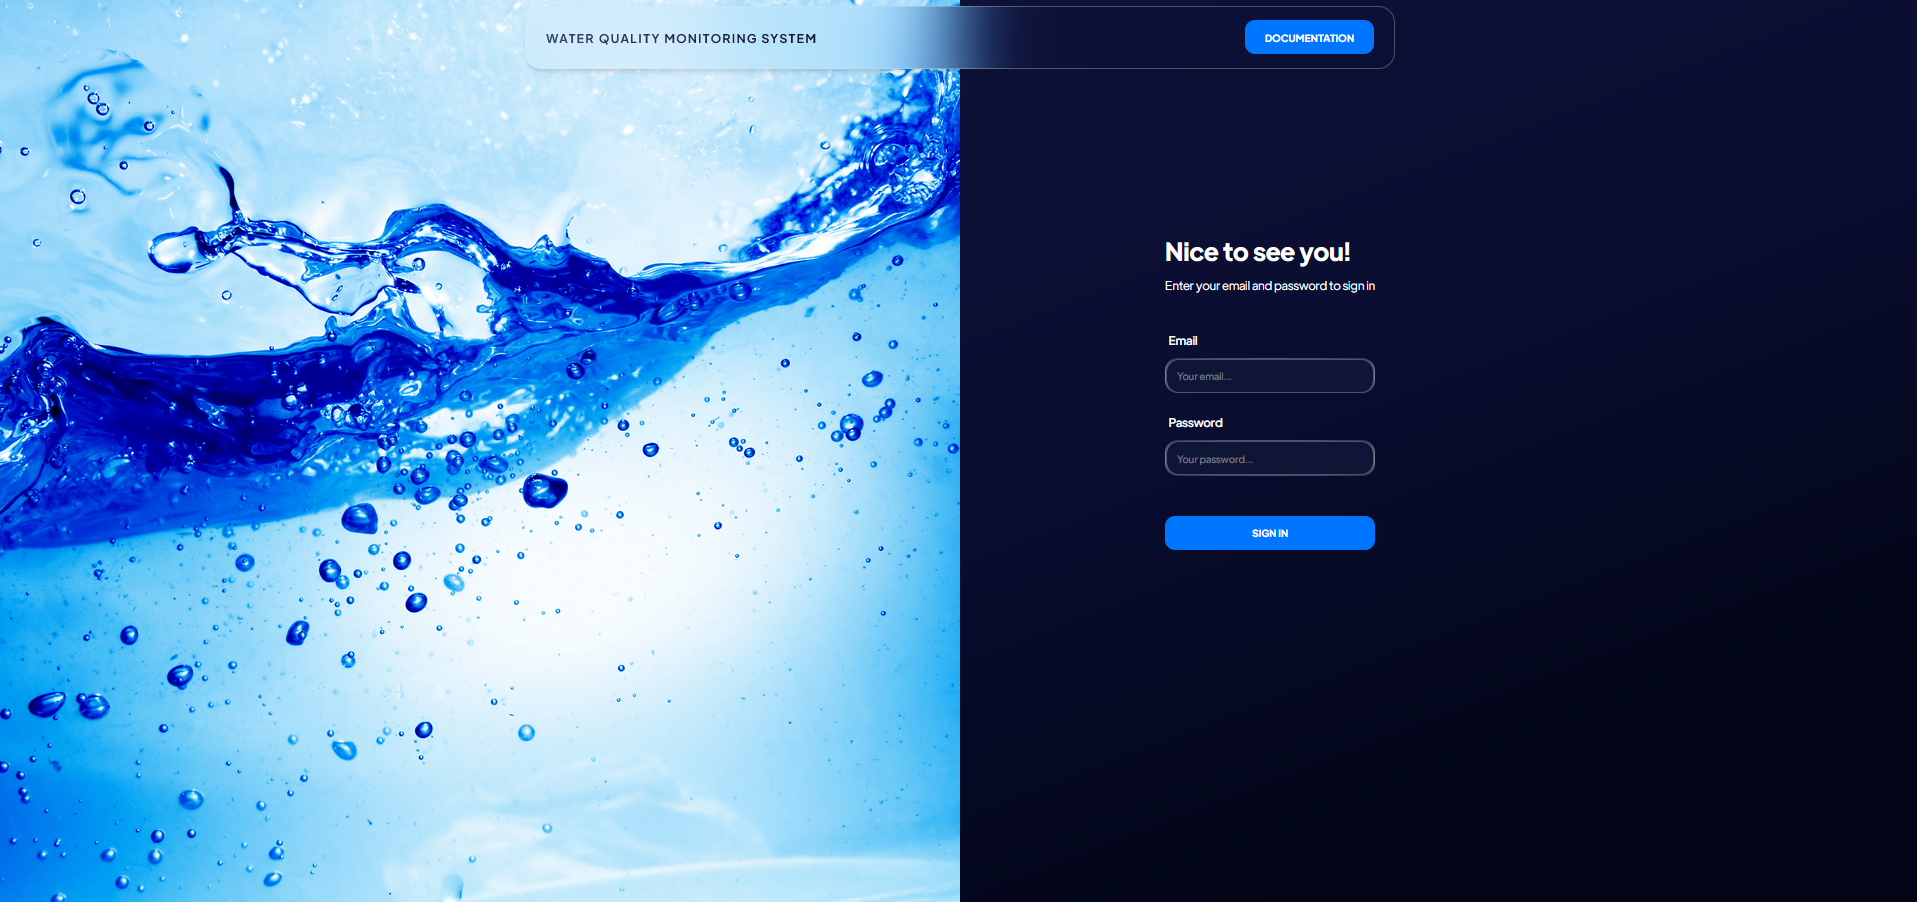
\includegraphics[width=0.75\linewidth]{Figures/admin1.png}
    \caption{Authentification Page}
    \label{fig:enter-label}
\end{figure}
The authentication page for the Water Quality Monitoring System features a straightforward login form, requesting the user's email and password. Notably, the system employs JWT  for secure user authentication. JWT ensures robust session management by generating encrypted tokens upon successful login.
\begin{figure}[H]
    \centering
    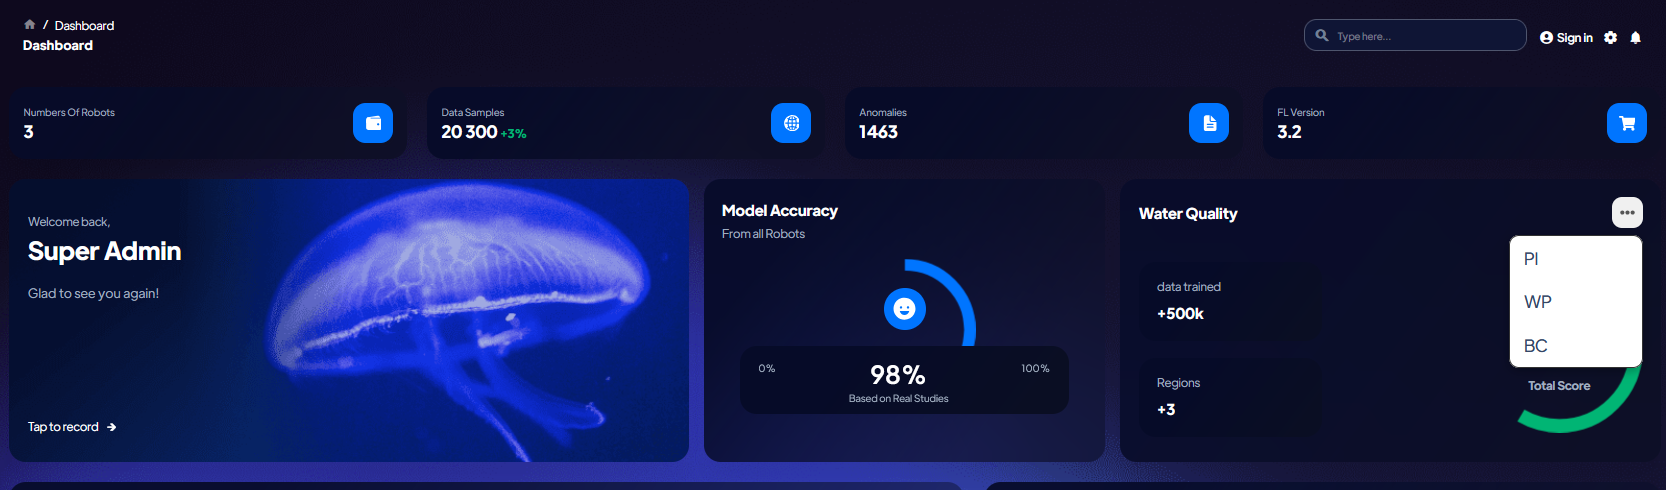
\includegraphics[width=0.75\linewidth]{Figures/admin2.png}
    \caption{Dashboard part 1}
    \label{fig:enter-label}
\end{figure}
This dashboard provides a unified view of business and environmental metrics, featuring admin analytics, service performance, and water quality data. Key sections include  number of active devices, model accuracy scores, and regional WQI trends with color-coded visuals. While effectively presenting diverse data, adding interactive elements could enhance usability.
\begin{figure}[H]
    \centering
    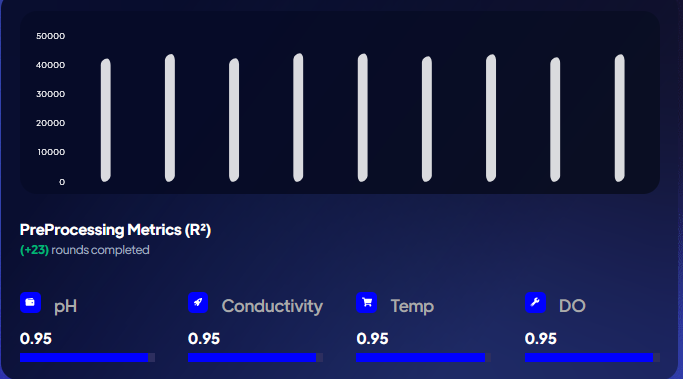
\includegraphics[width=0.75\linewidth]{Figures/admin3.png}
    \caption{Dashboard part 2}
    \label{fig:enter-label}
\end{figure}
This chart adopts a structured and minimalistic design to communicate model performance. The upper section features vertical bars that track outliers over time, visualizing monthly anomaly trends. The lower section presents accuracy scores across key water quality parameters, reflecting the strength of data cleaning models.

\begin{figure}[H]
    \centering
    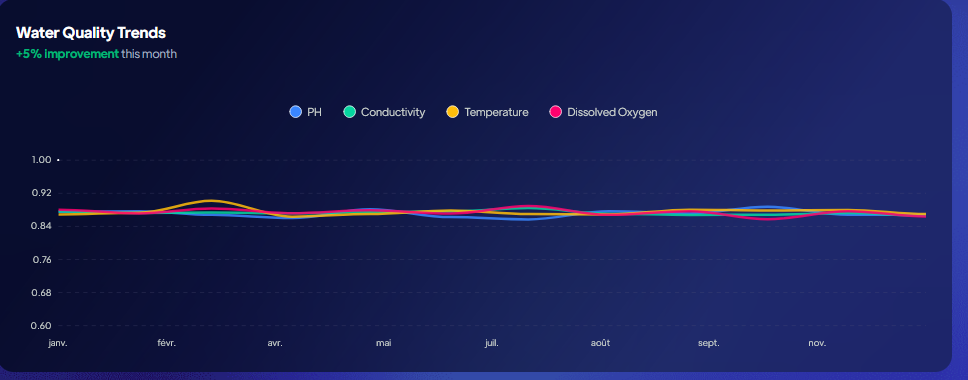
\includegraphics[width=0.75\linewidth]{Figures/dashboard4.png}
    \caption{Dashboard part 3}
    \label{fig:enter-label}
\end{figure}
This chart shows monthly trend lines for four water quality metrics. It displays percentage change data and tracks measurements across an eight-month period. The visualization uses a shared scale to compare the parameters, with time labels along the horizontal axis. A percentage indicator appears at the top. The chart presents the data clearly without interactive elements.
\begin{figure}[H]
    \centering
    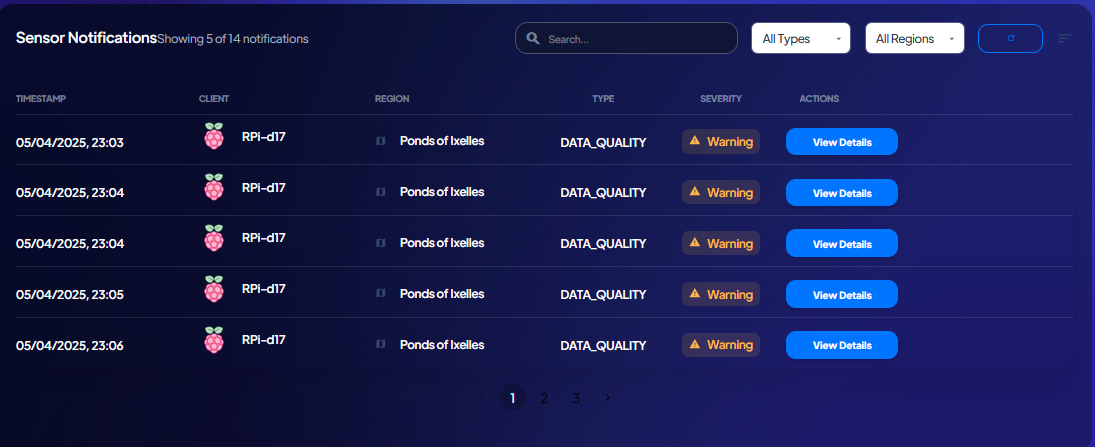
\includegraphics[width=0.75\linewidth]{Figures/admin5.png}
    \caption{dashboard part 4}
    \label{fig:enter-label}
\end{figure}
The interface displays a filterable notification log showing sensor alerts, including timestamps, locations, error types, and severity levels. It presents five entries for every page with options to sort by multiple columns and a search function. The visible alerts primarily show processing errors from one sensor location, with one data quality warning. Each entry includes an action button ("View Details") for further investigation.
\begin{figure}[H]
    \centering
    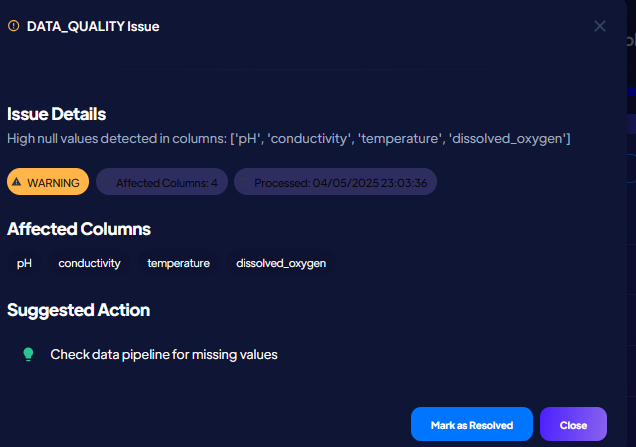
\includegraphics[width=0.7\linewidth]{Figures/admin8.png}
    \caption{dashboard part 5}
    \label{fig:enter-label}
\end{figure}

The interface displays a detailed data quality alert, showing affected measurement columns with null values. It includes the detection timestamp, severity level (warning), and recommended troubleshooting steps. The layout presents the information clearly with column headers, a suggested action prompt, and resolution options ("Mark as Resolved"/"Close").

\begin{figure}[H]
    \centering
    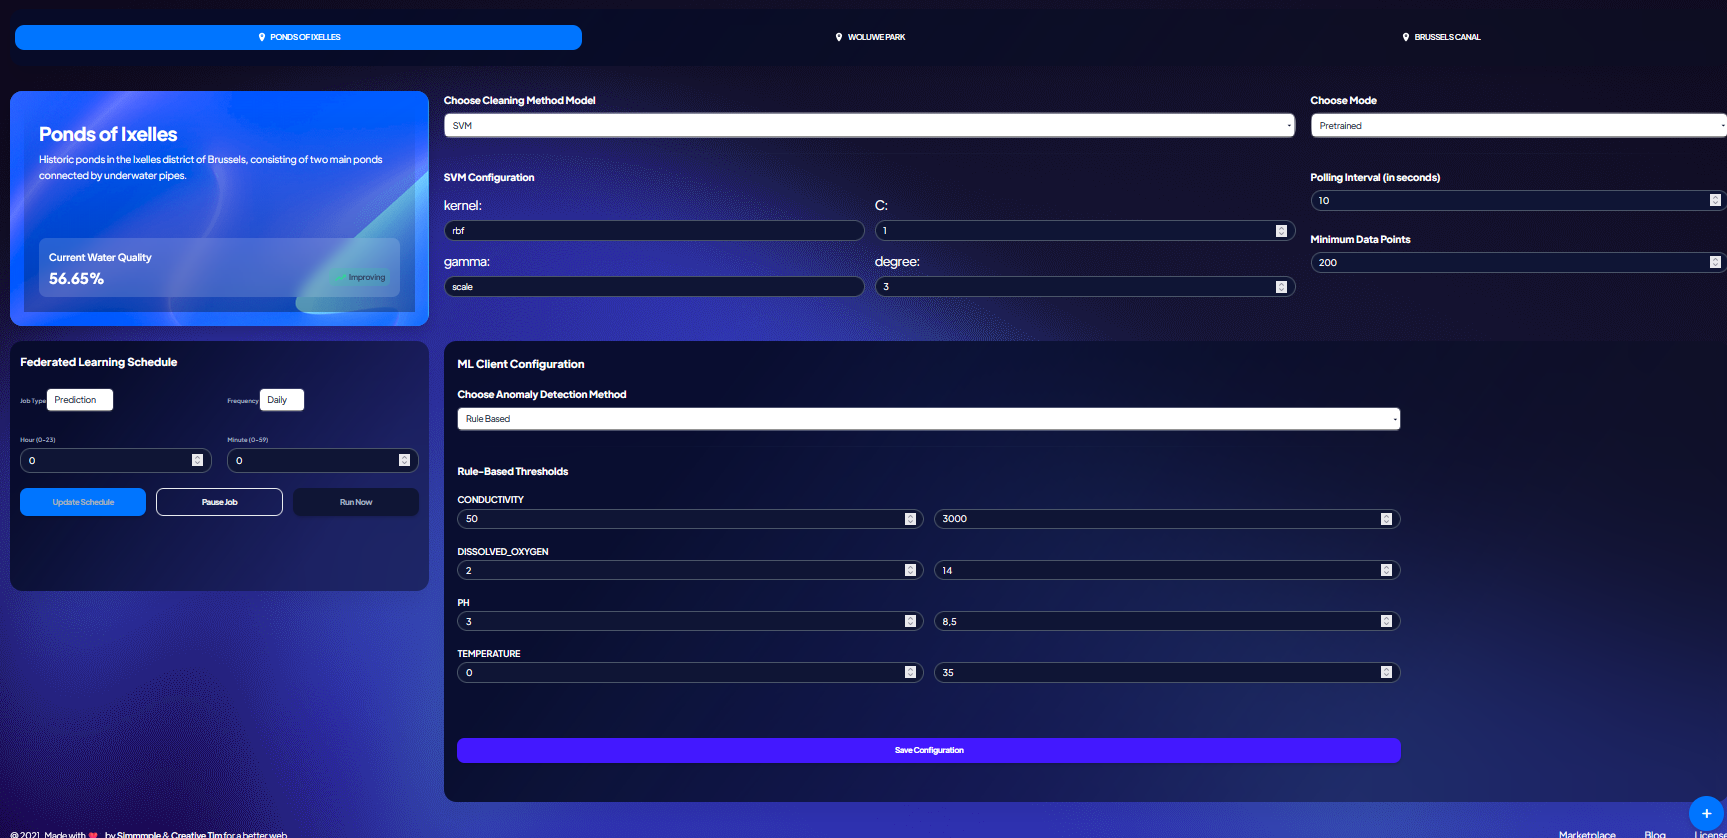
\includegraphics[width=0.75\linewidth]{Figures/configpage.png}
    \caption{Configurtion Page}
    \label{fig:enter-label}
\end{figure}


This Config panel provides an admin interface for comprehensively configuring a monitoring system., admin can select a "Cleaning Method Model" from a dropdown list (like SVM, KNN, RandomForest) and then input specific hyperparameter values for the chosen model into corresponding text fields or dropdowns. Similarly, for "ML Client Configuration," admin can choose an "Anomaly Detection Method" from a list (such as Rule-Based, IQR, Decision Tree). If "Rule-Based" is selected, the interface presents input fields to define numerical upper and lower thresholds for various sensor readings like conductivity, dissolved oxygen, pH, and temperature. If another method like Decision Tree were selected, different relevant parameter input fields would appear.
The interface also allows users to set general operational parameters like the "Polling Interval" and "Minimum Data Points" through numerical input fields, and select an operating "Mode" from a dropdown. For "Federated Learning Schedule," admin can select a "Job Type" (Prediction or Training), a "Frequency" (like Weekly, Monthly), and input specific times using hour and minute fields. Buttons for "Update Schedule," "Pause Job," and "Run Now" trigger corresponding backend actions. Finally, a "Save Configuration" button applies all the settings configured across these sections.

\begin{figure}[H]
    \centering
    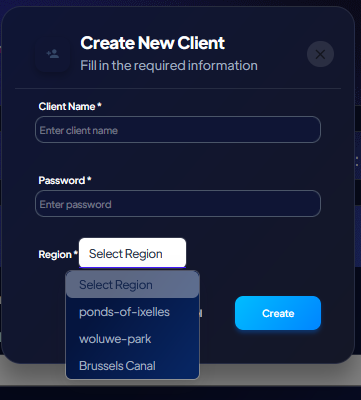
\includegraphics[width=0.5\linewidth]{Figures/create1.png}
    \caption{ Create Client Modal}
    \label{fig:enter-label}
\end{figure}
The interface shows a form for creating new device record, with required fields for name, password, and region selection. It includes a dropdown menu for choosing from predefined water monitoring locations. 
\begin{figure}[H]
    \centering
    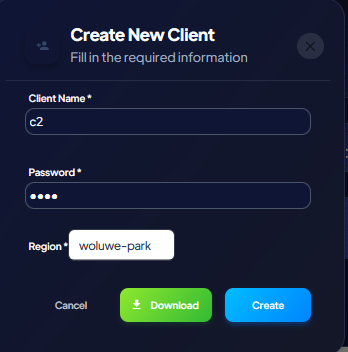
\includegraphics[width=0.5\linewidth]{Figures/create2.png}
    \caption{Enter Caption}
    \label{fig:enter-label}
\end{figure}

The interface displays a device creation form with fields for name, password, and region selection. After filling the form, a download button appears to retrieve security files (client.crt, client.key, ca.crt) packaged in a RAR archive.



\newpage

\section*{Conclusion}

This chapter comprehensively detailed the practical construction of the Federated Learning system for water quality monitoring, successfully translating architectural designs into a functional prototype. Key software components were developed and integrated, including mechanisms for data simulation, a robust preprocessing pipeline featuring anomaly detection and model-based cleaning, and the core federated learning workflow. Advanced analytical capabilities were implemented through dedicated feature engineering and the development of a Recurrent Neural Network model for water quality prediction. Security was a central focus, with mTLS and TLS protocols integrated to ensure secure communication across the system. Furthermore, user-facing client and administrator web interfaces were built using React.js with a Flask backend, providing essential tools for interaction, monitoring, and configuration. The successful amalgamation of these diverse elements into a working system demonstrates the viability of creating a sophisticated, privacy-preserving, and decentralized monitoring solution, thereby laying a solid groundwork for subsequent real-world testing and continued refinement.

\pagebreak